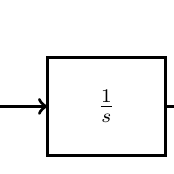
\begin{tikzpicture}[inner sep=0pt,outer sep=0pt,very thick,
sysblock/.style={draw,rectangle,inner sep=2pt,minimum width=1.5cm,minimum height=1.25cm,very thick}]
\useasboundingbox (-1,1) rectangle (0.5,-0.5); 
\begin{scope}[transform canvas={scale=1}]
\draw (0,0) node[sysblock] (S) {$\frac{1}{s}$};
\draw[->] (-2,0) node[above=2pt] {\textsf{Input}: $\frac{1}{s}$} -- (S.180);
\draw[->] (S.0) -- ++(2,0) node[above=2pt] {\textsf{Output}: $\frac{1}{s^2}$};
\end{scope}
\end{tikzpicture}
